\section{Introduction}
\label{sec:introduction}

% state the learning objective 
The objective of this laboratory assignment is to study a circuit containing a sinusodal voltage source $V_s$, a capacitor $C$,
a linear voltage dependent current source $I_b$, a linear current dependent voltage source $V_d$ and multiple resistors $R1,...,R7$.
The circuit can be seen in Figure~\ref{fig:lab2}.


In Section Theorical analysis and simulation results, the results of all the theoretical analysis of the circuit are
presented while comparing these to the ones obtained in ngspice simulation.
The conclusions of this study are outlined in Section Conclusion.

\begin{figure}[h] \centering
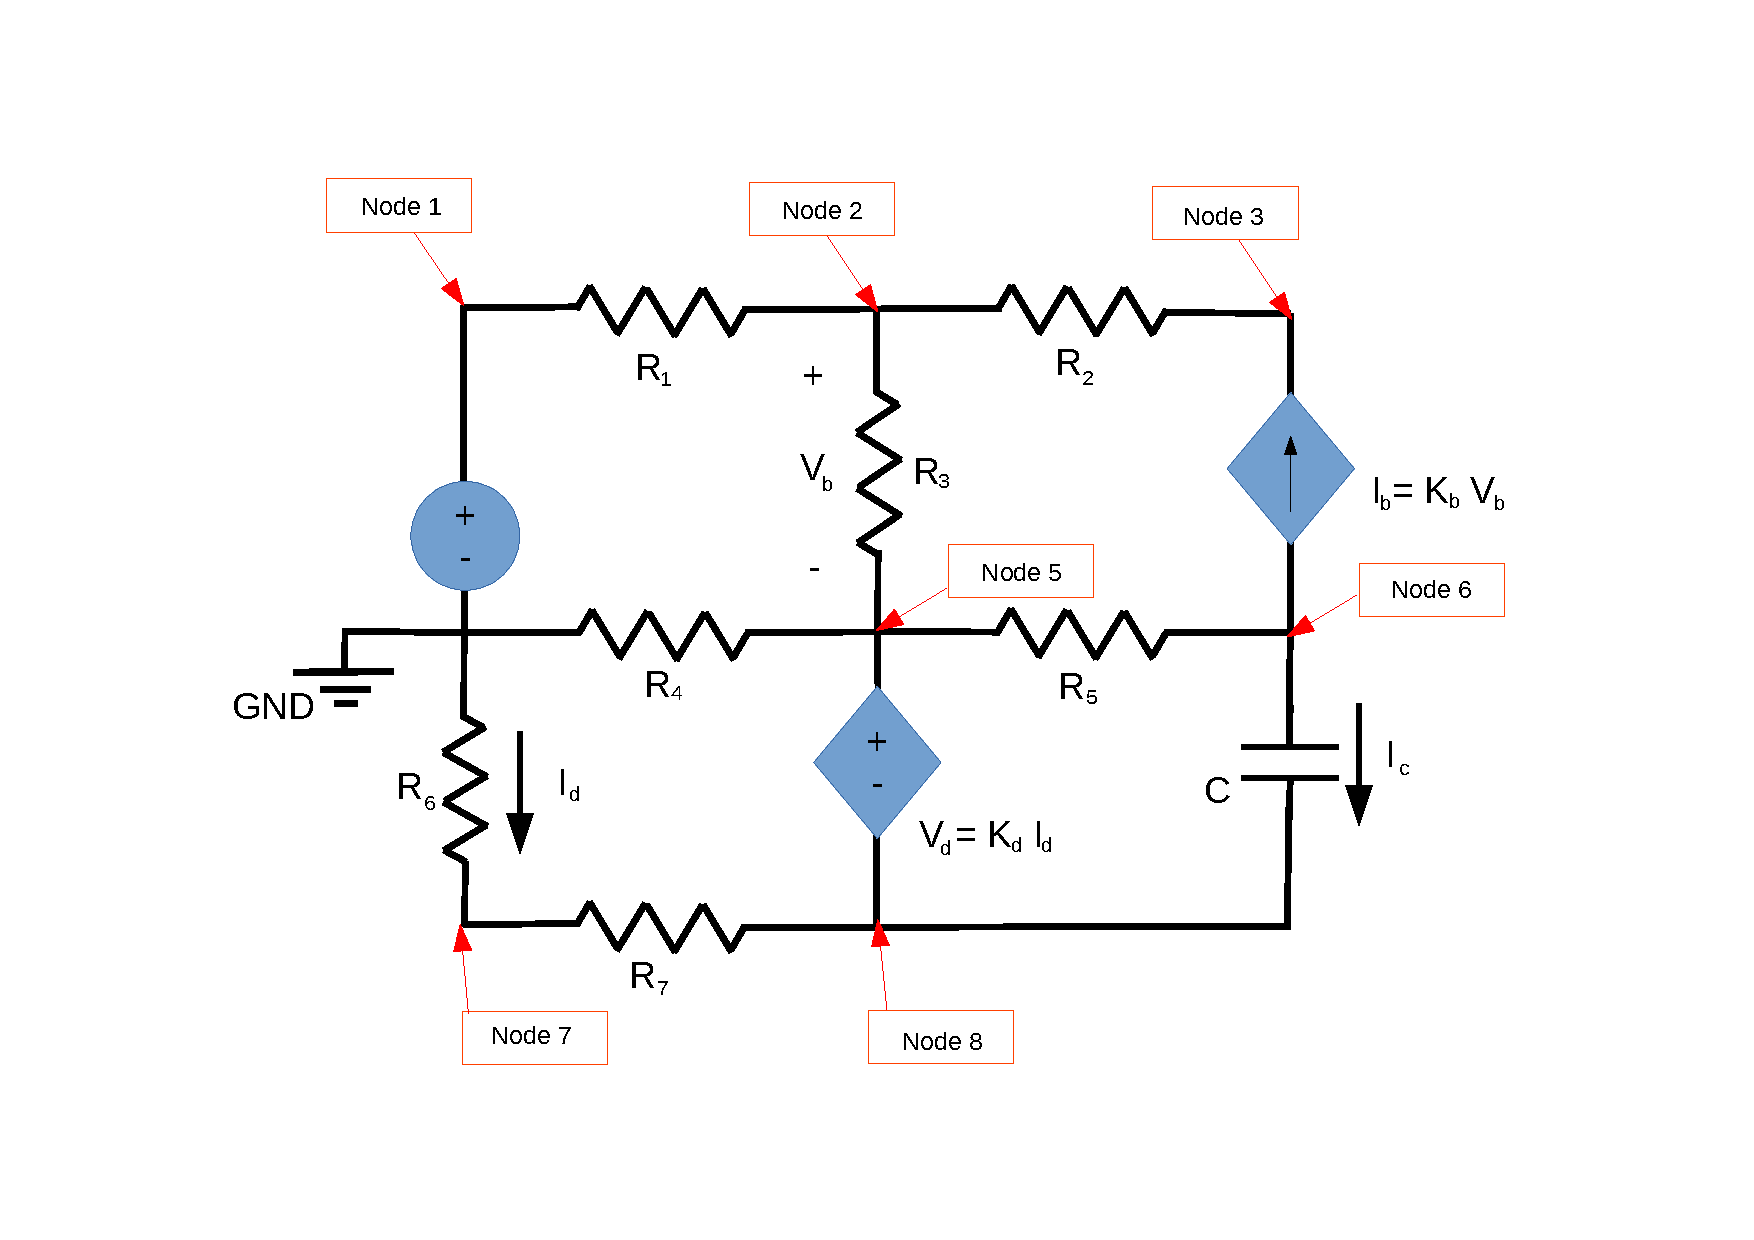
\includegraphics[width=1\linewidth]{../figlib/lab2.pdf}
\caption{Circuit to be analyzed in this report.}
\label{fig:lab2}
\end{figure}


